\documentclass[border=6pt]{standalone}
\usepackage{tikz}
\usetikzlibrary{arrows.meta, positioning, calc}

\definecolor{geno}{HTML}{0072B2}
\definecolor{pheno}{HTML}{D55E00}
\definecolor{fit}{HTML}{009E73}

\begin{document}
\pagecolor{white}
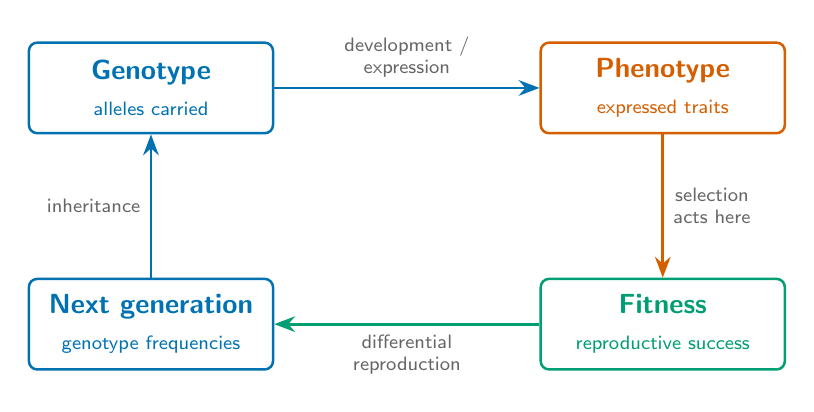
\begin{tikzpicture}[
    >=Stealth,
    font=\sffamily,
    box/.style={rounded corners=3pt, draw, line width=0.9pt, align=center,
                minimum width=3.1cm, minimum height=1.15cm},
    lab/.style={font=\sffamily\scriptsize, text=black!60, align=center},
    cyc/.style={->, line width=1.0pt},
]

\node[box, draw=geno, text=geno] (G) at (0,3)
    {\textbf{Genotype}\\[1pt]{\scriptsize alleles carried}};
\node[box, draw=pheno, text=pheno] (P) at (6.5,3)
    {\textbf{Phenotype}\\[1pt]{\scriptsize expressed traits}};
\node[box, draw=fit, text=fit] (F) at (6.5,0)
    {\textbf{Fitness}\\[1pt]{\scriptsize reproductive success}};
\node[box, draw=geno, text=geno] (O) at (0,0)
    {\textbf{Next generation}\\[1pt]{\scriptsize genotype frequencies}};

\draw[cyc, geno]  (G) -- (P) node[midway, above, lab] {development /\\ expression};
\draw[cyc, pheno] (P) -- (F) node[midway, right, lab] {selection\\ acts here};
\draw[cyc, fit]   (F) -- (O) node[midway, below, lab] {differential\\ reproduction};
\draw[cyc, geno]  (O) -- (G) node[midway, left, lab] {inheritance};

\end{tikzpicture}
\end{document}
